\documentclass[11pt]{article}

\usepackage[margin=1in]{geometry}
\usepackage[T1]{fontenc}
\usepackage{lmodern}
\usepackage{microtype}
\usepackage{amsmath,amssymb,amsthm}
\usepackage{booktabs}
\usepackage{siunitx}
\usepackage{xcolor}
\usepackage{tikz}
\usepackage{pgfplots}
\usepackage{caption}
\usepackage[section]{placeins}
\usepackage{subcaption}
\usepackage{algorithm}
\usepackage{algpseudocode}
\usepackage{listings}
\usepackage[colorlinks=true,linkcolor=blue!50!black,citecolor=blue!50!black,urlcolor=blue!50!black]{hyperref}
\usepackage[capitalise,noabbrev]{cleveref}

\pgfplotsset{compat=1.18}
\usetikzlibrary{arrows.meta,calc,patterns}

\sisetup{round-mode=figures,round-precision=3}

\lstset{basicstyle=\ttfamily\small,columns=fullflexible,keepspaces=true,
        frame=single,framerule=0.3pt,rulecolor=\color{black!30},
        backgroundcolor=\color{black!3},language=Fortran,
        keywordstyle=\color{blue!60!black},commentstyle=\color{green!40!black}}

\newcommand{\R}{\mathbb{R}}
\newcommand{\norm}[1]{\left\lVert #1 \right\rVert}
\newcommand{\code}[1]{\texttt{#1}}
\newcommand{\cond}{\kappa}
\DeclareMathOperator{\range}{range}
\DeclareMathOperator{\nnz}{nnz}

% plot styles for the solvers
\pgfplotscreateplotcyclelist{solvers}{%
  {black, mark=square*, mark size=1.6pt},
  {orange!80!black, mark=diamond*},
  {blue!70!black, mark=*,mark size=1.6pt},
  {cyan!60!black, mark=triangle*},
  {red!70!black, mark=pentagon*},
  {green!50!black, mark=star, thick},
}
\pgfplotsset{spy/.style={width=\linewidth, axis equal image, y dir=reverse,
  xmin=0.5, ymin=0.5, tick label style={font=\scriptsize}, title style={font=\small},
  enlargelimits=false}}

\title{\textbf{nlesolver-fortran}\\[0.3em]\large Theory, Options, and Performance of a Newton-Type Solver\\for Sparse and Dense Nonlinear Systems of Equations}
\author{Technical note}
\date{\today}

\begin{document}
\maketitle

\begin{abstract}
\noindent
\code{nlesolver-fortran} is a modern Fortran library for solving systems of $m$ nonlinear
equations in $n$ unknowns, $F(x) = 0$, where the system may be square ($m=n$),
underdetermined ($m<n$), or overdetermined ($m>n$), and the Jacobian may be dense or sparse.
This note describes the mathematical basis of the solver: the Newton--Raphson iteration and its
generalizations to non-square systems, the seven linear solvers available for computing the step
(including two built-in minimum-norm solvers, CRAIG and a sparse direct Cholesky method),
step-length control by line searches, Broyden and Schubert quasi-Newton updates, variable bounds,
and the stopping criteria. Numerical experiments with up to $500{,}000$ variables compare the
options, and the note ends with recommended settings for common use cases.
\end{abstract}

\tableofcontents
\newpage

%=============================================================================================
\section{Introduction}
%=============================================================================================

Many problems in engineering and science reduce to finding a point $x \in \R^n$ that satisfies
a set of nonlinear equations
\begin{equation}
  F(x) = \begin{bmatrix} f_1(x) & f_2(x) & \cdots & f_m(x) \end{bmatrix}^T = 0,
  \qquad F : \R^n \to \R^m .
  \label{eq:problem}
\end{equation}
Examples are trajectory design and targeting (where there are usually more free variables than
constraints), discretized boundary-value problems, and equilibrium calculations.

\code{nlesolver-fortran} solves \cref{eq:problem} with a Newton-type iteration. Its main features are:
\begin{itemize}
  \item square, underdetermined, and overdetermined systems;
  \item dense or sparse Jacobians, with a choice of seven linear solvers (\cref{sec:linear});
  \item four step-length strategies (\cref{sec:linesearch});
  \item optional Broyden (dense) or Schubert (sparse) Jacobian updates (\cref{sec:broyden});
  \item four modes for handling simple bounds on the variables (\cref{sec:bounds});
  \item a choice of the norm used to measure convergence (\cref{sec:stopping}).
\end{itemize}
The user supplies the function $F$ and its Jacobian
$J(x) = \partial F / \partial x \in \R^{m \times n}$, either as a dense array or as the nonzero
values of a fixed sparsity pattern.

\Cref{sec:newton} describes the Newton iteration for square and non-square systems.
\Cref{sec:linear} describes the linear solvers, \cref{sec:linesearch,sec:broyden,sec:bounds,sec:stopping}
the globalization, quasi-Newton, bounds, and stopping options.
\Cref{sec:experiments} presents numerical experiments, and \cref{sec:recommendations} gives
recommended settings. \Cref{sec:api} summarizes the interface.

%=============================================================================================
\section{The Newton iteration}
\label{sec:newton}
%=============================================================================================

Linearizing $F$ about the current iterate $x_k$ gives
\begin{equation}
  F(x_k + p) \approx F(x_k) + J(x_k)\, p .
\end{equation}
Setting the right-hand side to zero gives the \emph{Newton equations} for the step $p_k$:
\begin{equation}
  J_k\, p_k = -F_k, \qquad J_k = J(x_k),\; F_k = F(x_k),
  \label{eq:newton}
\end{equation}
and the next iterate is $x_{k+1} = x_k + \alpha_k p_k$, where the step length
$\alpha_k \in (0,1]$ is chosen by one of the strategies of \cref{sec:linesearch}.
The complete method is summarized in \cref{alg:newton}.

When $J_k$ is not square, \cref{eq:newton} does not have a unique solution, and the solver
uses the following generalization:
\begin{description}
  \item[Square ($m = n$):] $p_k = -J_k^{-1} F_k$. This is the classical Newton--Raphson method.
  If $J$ is nonsingular at a solution $x^*$ and Lipschitz continuous near it, the iteration
  converges quadratically from a close enough starting point:
  $\norm{x_{k+1} - x^*} \le C \norm{x_k - x^*}^2$ \cite{dennis_schnabel}.

  \item[Underdetermined ($m < n$):] \cref{eq:newton} has infinitely many solutions (if $J_k$ has
  full row rank). The solver uses the \emph{minimum-norm} step
  \begin{equation}
    p_k = \arg\min_p \norm{p}_2 \quad \text{subject to} \quad J_k p = -F_k,
    \qquad\text{i.e.}\qquad p_k = -J_k^{+} F_k = -J_k^T (J_k J_k^T)^{-1} F_k,
    \label{eq:minnorm}
  \end{equation}
  where $J^+$ is the Moore--Penrose pseudoinverse. This is the Newton method of
  Ben-Israel \cite{benisrael1966}; with $J$ of full row rank near the solution set it also converges
  quadratically to \emph{a} solution \cite{levin_benisrael}. The solutions of an underdetermined system
  form an $(n-m)$-dimensional manifold $\mathcal{M} = \{x : F(x) = 0\}$, and the minimum-norm step is
  the shortest step to the linearization of $\mathcal{M}$.

  \item[Overdetermined ($m > n$):] \cref{eq:newton} usually has no solution, and the solver uses the
  least-squares step
  \begin{equation}
    p_k = \arg\min_p \norm{J_k p + F_k}_2 = -(J_k^T J_k)^{-1} J_k^T F_k ,
  \end{equation}
  which is the Gauss--Newton method for $\min_x \tfrac12 \norm{F(x)}_2^2$. It converges quadratically
  only when the residual at the solution is zero.
\end{description}

\begin{algorithm}[t]
\caption{Newton iteration in \code{nlesolver-fortran} (simplified).}
\label{alg:newton}
\begin{algorithmic}[1]
\State project $x_0$ onto the bounds (if any); $F_0 \gets F(x_0)$; $f_0 \gets \norm{F_0}$
\If{$f_0 \le \code{tol}$} \Return $x_0$ \EndIf
\For{$k = 0, 1, \ldots, \code{max\_iter}-1$}
  \State $J_k \gets J(x_k)$ \Comment{or a Broyden/Schubert update, \cref{sec:broyden}}
  \State solve $J_k p_k = -F_k$ for the step $p_k$ \Comment{\cref{sec:linear}}
  \State adjust $p_k$ for the bounds \Comment{\cref{sec:bounds}}
  \State choose $\alpha_k$; $x_{k+1} \gets x_k + \alpha_k p_k$; $F_{k+1} \gets F(x_{k+1})$
         \Comment{\cref{sec:linesearch}}
  \If{$f_{k+1} \le \code{tol}$} \Return $x_{k+1}$ (converged) \EndIf
  \If{$\max_i |x_{k+1,i} - x_{k,i}| \le \code{tolx}$} \Return $x_{k+1}$ (no progress) \EndIf
  \If{more than \code{n\_uphill\_max} consecutive increases of $f$} \Return \EndIf
\EndFor
\end{algorithmic}
\end{algorithm}

\paragraph{Minimum-norm steps and the closest solution.}
For a linear underdetermined system, the minimum-norm step from $x_0$ lands on the solution
closest to $x_0$. For a nonlinear system this is not true in general: each step $p_k$ is normal
to the level sets of $F$ at $x_k$, but the closest point $x^\dagger$ of $\mathcal{M}$ to $x_0$ is
characterized by
\begin{equation}
  x^\dagger - x_0 \in \range\!\big(J(x^\dagger)^T\big),
  \label{eq:closest}
\end{equation}
i.e.\ the total displacement must be normal to $\mathcal{M}$ at $x^\dagger$, while
$x_k - x_0 = \sum_j \alpha_j p_j$ with $p_j \in \range(J(x_j)^T)$. \Cref{fig:parabola} shows the
difference for the single equation $y - x^2 = 0$. If the closest solution is required, each step
can instead be computed from
$\min_p \norm{x_k + p - x_0}$ subject to $J_k p = -F_k$, which is a minimum-norm problem for
$q = p + (x_k - x_0)$ with right-hand side $-F_k + J_k (x_k - x_0)$. (This option is not
currently implemented; see \cref{sec:future}.)

\begin{figure}[htbp]
\centering
\begin{tikzpicture}
\begin{axis}[width=0.55\textwidth, axis equal image,
  xmin=0.3, xmax=1.1, ymin=-0.05, ymax=0.5, xlabel={$x$}, ylabel={$y$},
  legend pos=outer north east, legend style={font=\small}, legend cell align=left]
  \addplot[domain=0.3:0.72, samples=60, gray, thick] {x^2};
  \addlegendentry{$\mathcal{M}: y = x^2$}
  \addplot[blue!70!black, mark=*, mark size=1.5pt] table[x=x,y=y,col sep=comma] {data/parabola_plain.csv};
  \addlegendentry{minimum-norm Newton iterates}
  \addplot[red!70!black, dashed, mark=o, mark size=1.5pt] table[x=x,y=y,col sep=comma] {data/parabola_anchored.csv};
  \addlegendentry{anchored iterates (closest point)}
  \addplot[only marks, mark=star, mark size=4pt, green!50!black, thick] table[x=x,y=y,col sep=comma] {data/parabola_closest.csv};
  \addlegendentry{closest point to $x_0$}
  \node[anchor=west] at (axis cs:1.0,0.0) {$x_0$};
  \draw[green!50!black, densely dotted] (axis cs:1,0) -- (axis cs:0.5897545,0.3478104);
\end{axis}
\end{tikzpicture}
\caption{Minimum-norm Newton iterates for $F(x,y) = y - x^2$ from $x_0 = (1,0)$ converge to
$(0.518, 0.269)$, at distance $0.5516$ from $x_0$. The closest solution is $(0.590, 0.348)$, at
distance $0.5378$. The ``anchored'' iteration of \cref{sec:newton} converges to the closest point.}
\label{fig:parabola}
\end{figure}

%=============================================================================================
\section{Linear solvers for the Newton step}
\label{sec:linear}
%=============================================================================================

Computing the step \cref{eq:newton} is usually the most expensive part of an iteration.
The linear solver is selected with \code{sparsity\_mode}; \cref{tab:solvers} summarizes the
options. For the sparse modes the Jacobian is given in coordinate (triplet) form: the user
supplies the row and column indices of the $\nnz$ nonzeros once (\code{irow}, \code{icol}), and the
Jacobian routine returns their values in the same order.

\begin{table}[htbp]
\centering
\caption{Linear solvers (\code{sparsity\_mode}). ``Min-norm'' is the solution of \cref{eq:minnorm};
``LS'' the least-squares solution. Damping is described in \cref{sec:damping}.}
\label{tab:solvers}
\small
\begin{tabular}{@{}clllll@{}}
\toprule
mode & solver & type & $m<n$ & $m>n$ & damping \\
\midrule
1 & dense LAPACK (\code{dgesv}/\code{dgels}) & direct & min-norm & LS & no \\
2 & LSQR \cite{lsqr} & iterative & min-norm\textsuperscript{a} & LS & yes \\
3 & LUSOL \cite{lusol} & direct (sparse LU) & no\textsuperscript{b} & no\textsuperscript{b} & no \\
4 & LSMR \cite{lsmr} & iterative & min-norm\textsuperscript{a} & LS & yes \\
5 & user-supplied & -- & -- & -- & -- \\
6 & CRAIG (built in) & iterative & min-norm & no\textsuperscript{c} & yes \\
7 & sparse Cholesky of $JJ^T$ (built in) & direct & min-norm & no\textsuperscript{c} & yes \\
\bottomrule
\end{tabular}

\vspace{0.3em}
\begin{minipage}{0.9\textwidth}\footnotesize
\textsuperscript{a} For a compatible system and a zero starting vector (as used by the solver).\quad
\textsuperscript{b} Square systems only: for $m<n$ LUSOL reports the system as singular
(\cref{sec:exp-scaling}).\quad
\textsuperscript{c} Requires $J J^T$ nonsingular, i.e.\ $J$ of full row rank, which is not possible
for $m>n$ (unless \code{damp}${}>0$).
\end{minipage}
\end{table}

\subsection{Dense solver (mode 1)}
For $m = n$ the step is computed with an LU factorization with partial pivoting (LAPACK
\code{dgesv}). For $m \ne n$, LAPACK \code{dgels} is used: a QR factorization of $J$ for $m > n$
(least squares) and an LQ factorization for $m < n$ (minimum norm). The cost is
$O(m n \min(m,n))$ operations and $mn$ storage per iteration, so this mode is limited to a few
thousand variables.

\subsection{LUSOL (mode 3)}
LUSOL \cite{lusol} computes a sparse LU factorization $P J Q = L U$ with threshold pivoting
(\code{lusol\_method}: threshold partial, rook, or complete pivoting) that balances sparsity
against stability. It is a fast and robust choice for square systems. As used by the solver it is
not suitable for rectangular systems: for $m < n$ the factorization reports the matrix as singular
(rank $m$, with $n-m$ ``singularities'') and the Newton iteration fails.

\subsection{Golub--Kahan bidiagonalization}
The three iterative solvers (LSQR, LSMR, CRAIG) are all based on the Golub--Kahan
bidiagonalization of $A = J_k$ with starting vector $b = -F_k$:
\begin{equation}
\begin{aligned}
  \beta_1 u_1 &= b, & \alpha_1 v_1 &= A^T u_1, \\
  \beta_{i+1} u_{i+1} &= A v_i - \alpha_i u_i, & \alpha_{i+1} v_{i+1} &= A^T u_{i+1} - \beta_{i+1} v_i ,
\end{aligned}
\label{eq:gk}
\end{equation}
where the scalars $\alpha_i, \beta_i \ge 0$ normalize the vectors. After $k$ steps,
$U_k = [u_1 \cdots u_k]$ and $V_k = [v_1 \cdots v_k]$ have orthonormal columns (in exact arithmetic) and
\begin{equation}
  A V_k = U_k L_k + \beta_{k+1} u_{k+1} e_k^T, \qquad A^T U_k = V_k L_k^T,
  \qquad
  L_k = \begin{bmatrix} \alpha_1 \\ \beta_2 & \alpha_2 \\ & \ddots & \ddots \\ && \beta_k & \alpha_k \end{bmatrix}.
\end{equation}
Each step costs one product with $A$ and one with $A^T$, i.e.\ $O(\nnz)$ operations, and only a few
vectors of length $m$ and $n$ are stored. The three methods differ in what they minimize over
the Krylov subspace $\range(V_k)$:
\begin{itemize}
  \item \textbf{LSQR} \cite{lsqr} minimizes the residual $\norm{b - A x_k}$;
  \item \textbf{LSMR} \cite{lsmr} minimizes $\norm{A^T(b - A x_k)}$, which decreases monotonically and
  allows earlier stopping for least-squares problems. LSMR can optionally reorthogonalize the
  most recent \code{localSize} vectors $v_i$;
  \item \textbf{CRAIG} \cite{saunders1995} minimizes the error $\norm{x^\dagger - x_k}$, where $x^\dagger$
  is the minimum-norm solution of a compatible system.
\end{itemize}
Starting from $x_0 = 0$, all iterates lie in $\range(A^T)$, so for a compatible system each of the three
converges to the minimum-norm solution.

\subsection{CRAIG (mode 6)}
\label{sec:craig}
CRAIG takes $x_k = V_k z_k$ with $L_k z_k = \beta_1 e_1$. Since $L_k$ is lower bidiagonal, $z_k$
is obtained by forward substitution, one element per iteration:
\begin{equation}
  \zeta_1 = \frac{\beta_1}{\alpha_1}, \qquad \zeta_k = -\frac{\beta_k\, \zeta_{k-1}}{\alpha_k},
  \qquad x_k = x_{k-1} + \zeta_k v_k .
\end{equation}
Using \cref{eq:gk}, the residual is
$r_k = b - A x_k = -\beta_{k+1} \zeta_k u_{k+1}$, so its norm $\norm{r_k} = |\beta_{k+1}\zeta_k|$
is available at no cost. The iteration stops when
\begin{equation}
  \norm{r_k} \le \code{btol}\,\norm{b} + \code{atol}\,\norm{A}_F \norm{x_k},
\end{equation}
or after \code{itnlim} iterations. CRAIG is mathematically equivalent to the conjugate gradient
method applied to $A A^T y = b$, $x = A^T y$ (``CGNE''), but does not form $A A^T$. Its convergence
is therefore governed by $\cond(A A^T) = \cond(A)^2$: the error is reduced by a fixed factor in
$O(\cond(A))$ iterations \cite{saunders1995}. If $\alpha_k = 0$ the system is incompatible and the
method stops with an error (status $-1007$).

\subsection{Sparse direct minimum-norm solver (mode 7)}
\label{sec:cholesky}
The minimum-norm solution can also be written as the solution of the ``normal equations of the
second kind''
\begin{equation}
  (A A^T + \delta^2 I)\, y = b, \qquad x = A^T y ,
  \label{eq:normal2}
\end{equation}
where $\delta$ is the damping parameter (\cref{sec:damping}; $\delta = 0$ by default). The
$m \times m$ matrix $B = A A^T + \delta^2 I$ is symmetric positive definite when $A$ has full row
rank (or $\delta > 0$), and $B_{ij} \neq 0$ only if rows $i$ and $j$ of $A$ share a column.
Mode 7 solves \cref{eq:normal2} with a sparse Cholesky factorization $P B P^T = L L^T$ in three phases:

\begin{enumerate}
\item \textbf{Analysis} (once per sparsity pattern). The graph of $B$ (rows connected if they share
a column) is formed, and the rows are reordered with the \emph{reverse Cuthill--McKee} (RCM)
algorithm \cite{cuthill_mckee,george_liu}: a breadth-first search from a pseudo-peripheral node,
visiting neighbors in order of increasing degree, then reversed. RCM makes the nonzeros of $P B P^T$
cluster near the diagonal. The \emph{envelope} of row $r$ is the range of columns
$f_r \le j \le r$, where $f_r$ is the first nonzero column of row $r$; since all fill-in of a Cholesky
factorization stays inside the envelope, $L$ is stored row by row in
$\sum_r (r - f_r + 1)$ locations (``skyline'' storage), and no further symbolic analysis is needed.

\item \textbf{Factorization} (each iteration). $B$ is formed directly in the envelope storage from the
sparse rows of $A$ (each row of $A$ is scattered into a work vector of length $n$, and sparse dot
products with the adjacent rows give the entries of $B$), so neither $A$ nor $B$ is ever formed as a
dense matrix. Then a row-oriented envelope Cholesky factorization is done in place:
\begin{equation}
  L_{rq} = \frac{1}{L_{qq}}\Big( B_{rq} - \sum_{j=\max(f_r,f_q)}^{q-1} L_{rj} L_{qj} \Big), \quad f_r \le q < r,
  \qquad
  L_{rr} = \Big( B_{rr} - \sum_{j=f_r}^{r-1} L_{rj}^2 \Big)^{1/2}.
\end{equation}
The inner sums are dot products of contiguous segments, which vectorize well. A pivot
$L_{rr}^2 \le 4\epsilon B_{rr}$ indicates that $A$ is (numerically) rank deficient, and the solver
stops with status $-1008$ (use $\delta > 0$).

\item \textbf{Solve} (each iteration). Forward and back substitution with $L$ give $y$, then
$x = A^T y$.
\end{enumerate}

\paragraph{Cost.}
If $w$ is the (average) half-bandwidth of $P B P^T$, the factorization costs $O(m w^2)$ operations and
$O(m w)$ storage. For a Jacobian in which each equation involves a band of nearby variables (even if
the equations are numbered arbitrarily), $w$ is a small constant and the solver is very fast. For
Jacobians with 2-D or 3-D ``mesh-like'' coupling, $w$ grows like $m^{1/2}$ or $m^{2/3}$ and the envelope
contains many zeros (\cref{sec:exp-sparsity}).

\paragraph{Accuracy and iterative refinement.}
Forming $B = A A^T$ squares the condition number, $\cond(B) = \cond(A)^2$, so the computed $y$ can
have a relative error of order $\epsilon\, \cond(A)^2$. Moreover, for an ill-conditioned $A$, $y$ can be
very large while $x = A^T y$ is not, so computing $x$ from $y$ involves cancellation. The solver
therefore uses iterative refinement with the residual of the original system:
\begin{equation}
  r = b - A x - \delta^2 y, \qquad
  B\, \Delta y = r \;(\text{using } L), \qquad
  y \gets y + \Delta y, \qquad x \gets x + A^T \Delta y .
\end{equation}
Accumulating $x$ directly (rather than recomputing $A^T y$) avoids the cancellation, since the
corrections $\Delta y$ become small. Each correction lies in $\range(A^T)$, so the minimum-norm
property is kept. The refinement contracts the error by a factor of about $c\,\epsilon\,\cond(A)^2$ per
step, so it converges for $\cond(A) \lesssim 10^{8}$ in double precision. At most
\code{cholesky\_refine} steps are taken (default 2), and the refinement stops early if the residual
stops decreasing.

\subsection{Damping and regularization}
\label{sec:damping}
LSQR, LSMR, CRAIG, and the Cholesky solver accept a damping parameter $\delta = \code{damp} \ge 0$.
LSQR and LSMR solve $\min_x \norm{Ax - b}^2 + \delta^2 \norm{x}^2$, and CRAIG solves
$\min \norm{x}^2 + \norm{s}^2$ subject to $Ax + \delta s = b$ (by applying the method to
$[A,\ \delta I]$); like \cref{eq:normal2}, both give
\begin{equation}
  x(\delta) = (A^T A + \delta^2 I)^{-1} A^T b = A^T (A A^T + \delta^2 I)^{-1} b .
\end{equation}
For the Newton step this is a Levenberg--Marquardt step with a fixed parameter
$\lambda = \delta^2$: $p = \arg\min_p \norm{J_k p + F_k}^2 + \delta^2 \norm{p}^2$. Damping makes
the step well defined when $J_k$ is rank deficient, and shortens it, at the cost of slower
convergence near the solution (the step is no longer an exact Newton step). As $\delta \to 0$,
$x(\delta)$ tends to the minimum-norm solution.

\subsection{User-supplied solver (mode 5)}
A procedure with the interface \code{sparse\_solver\_func} receives the sparse Jacobian and
right-hand side and returns the step. This can be used to call external libraries, for example
qr\_mumps \cite{qrmumps} or SuiteSparseQR, for problems with general sparsity.

%=============================================================================================
\section{Step length control}
\label{sec:linesearch}
%=============================================================================================

The full Newton step ($\alpha_k = 1$) converges quickly near a solution but may diverge from a poor
starting point. The step length is chosen by \code{step\_mode} within
$[\alpha_{\min}, \alpha_{\max}] \subseteq (0,1]$ (defaults $0.1$ and $1$). The line searches use the merit
function
\begin{equation}
  \phi(\alpha) = \tfrac12 \norm{F(x_k + \alpha p_k)}_2^2 ,
  \qquad
  \phi'(0) = p_k^T J_k^T F_k ,
  \label{eq:merit}
\end{equation}
where $\phi'(0)$ is computed with the chain rule from the current Jacobian (for a sparse Jacobian
directly from the triplets, in $O(\nnz)$ operations). If $p_k$ solves $J_k p_k = -F_k$ exactly,
$\phi'(0) = -\norm{F_k}^2 < 0$, so $p_k$ is a descent direction for $\phi$.

\begin{description}
\item[Mode 1: constant step.] $\alpha_k = \code{alpha}$ (default 1). The cheapest option: one function
evaluation per iteration. Pure Newton for $\code{alpha}=1$.

\item[Mode 2: backtracking.] Starting from $\alpha = \alpha_{\max}$, $\alpha$ is reduced by the factor
$\tau$ (default $0.5$) until the Armijo sufficient-decrease condition
\begin{equation}
  \phi(\alpha) \le \phi(0) + c\, \alpha\, \phi'(0)
  \label{eq:armijo}
\end{equation}
holds, or $\alpha_{\min}$ is reached. The constant $c$ (\code{backtrack\_c}, default $10^{-4}$) must be
less than $\tfrac12$: near a solution, $\phi(1) = O(\norm{F_k}^4)$, while \cref{eq:armijo} with $\alpha=1$
requires $\phi(1) \le (1-2c)\,\phi(0)$, so for $c < \tfrac12$ the full Newton step is eventually always
accepted and quadratic convergence is kept.

\item[Mode 3: ``exact'' line search.] $\alpha_k$ minimizes $\norm{F(x_k + \alpha p_k)}^2$ over
$[\alpha_{\min}, \alpha_{\max}]$ using Brent's method \cite{brent} (\code{fmin}) with tolerance
\code{fmin\_tol}. The full step $\alpha_{\max}$ is also evaluated, since Brent's method never evaluates
the ends of the interval, and near a solution the full step is usually the minimizer. Minimizing the
squared norm (rather than the norm) gives the same minimizer, but a smooth function at a root, which
suits Brent's parabolic interpolation. Costs about $10$--$20$ function evaluations per iteration.

\item[Mode 4: fixed points.] $F$ is evaluated at $\code{n\_intervals}+1$ equally spaced values of
$\alpha$ in $[\alpha_{\min}, \alpha_{\max}]$, and the best one is taken. Simple and robust; a fixed cost
of $\code{n\_intervals}+1$ function evaluations per iteration.
\end{description}

\noindent
Note that no line search can guarantee a decrease if $p_k$ is not a descent direction (for example
with an inaccurate Broyden Jacobian), since $\alpha_{\min} > 0$. The iteration then counts ``uphill''
steps and stops after \code{n\_uphill\_max} consecutive increases (status 5); with Broyden updates, an
uphill step also triggers a new Jacobian evaluation.

%=============================================================================================
\section{Quasi-Newton updates}
\label{sec:broyden}
%=============================================================================================

If the Jacobian is expensive, \code{use\_broyden = .true.} replaces most Jacobian evaluations by a
secant update. With $\Delta x = x_{k+1} - x_k$ and $\Delta F = F_{k+1} - F_k$:

\paragraph{Broyden (dense).} The ``good'' Broyden update \cite{broyden} is the smallest change to
$J_k$ (in the Frobenius norm) that satisfies the secant equation $J_{k+1} \Delta x = \Delta F$:
\begin{equation}
  J_{k+1} = J_k + \frac{(\Delta F - J_k \Delta x)\, \Delta x^T}{\Delta x^T \Delta x} .
\end{equation}

\paragraph{Schubert (sparse).} The Broyden update fills in the Jacobian. Schubert's update
\cite{schubert} applies the same idea row by row, using only the variables in the sparsity pattern
of each row. With $\Delta x^{(i)}$ the vector $\Delta x$ with the components outside the pattern of
row $i$ set to zero:
\begin{equation}
  J_{k+1}(i,:) = J_k(i,:) + \frac{\big(\Delta F_i - J_k(i,:)\, \Delta x\big)\, \Delta x^{(i)T}}{\Delta x^{(i)T} \Delta x^{(i)}} .
\end{equation}
The nonzeros are grouped by row once, so each update costs $O(\nnz)$. A row whose variables did not
change ($\Delta x^{(i)} \approx 0$) is left unchanged.

\paragraph{Resets.} The true Jacobian is evaluated at the first iteration, after
\code{broyden\_update\_n} consecutive updates (default 4; 0 means never), after an uphill step, and when
$\norm{\Delta x}^2 \le \epsilon$. Quasi-Newton updates trade more iterations (superlinear instead of
quadratic convergence) for fewer Jacobian evaluations; they pay off when a Jacobian evaluation costs
much more than a function evaluation plus a linear solve (\cref{sec:exp-steps}).

%=============================================================================================
\section{Variable bounds}
\label{sec:bounds}
%=============================================================================================

Simple bounds $x_\ell \le x \le x_u$ are handled by modifying the step; four modes are available
(\code{bounds\_mode}), illustrated in \cref{fig:bounds}. In all modes the initial point is first
projected onto the bounds. Let $\tilde x = x_k + p_k$ be the full Newton point.
\begin{description}
  \item[0: ignore] the bounds (default).
  \item[1: scalar.] Each violating component of $\tilde x$ is moved to its bound, and the step becomes
  $\tilde p = \operatorname{clip}(\tilde x) - x_k$. Both the direction and the length can change.
  \item[2: vector.] The step is shortened along the Newton direction:
  $\tilde p = t\, p_k$ with
  \begin{equation}
     t = \min_{i:\ \tilde x_i \notin [x_{\ell,i},\, x_{u,i}]} \frac{b_i - x_{k,i}}{p_{k,i}},
     \qquad b_i \in \{x_{\ell,i}, x_{u,i}\}\ \text{the violated bound},
  \end{equation}
  so the direction is preserved.
  \item[3: wall.] As the scalar mode, but the components put on the bounds stay there during the line
  search: $x(\alpha)_i = b_i$ for those components, and $x_{k,i} + \alpha \tilde p_i$ for the others.
\end{description}
The vector mode keeps the Newton direction (and its descent property) but can produce very short steps
when a single variable is near its bound. The scalar and wall modes let the other variables continue to
move.

\begin{figure}[htbp]
\centering
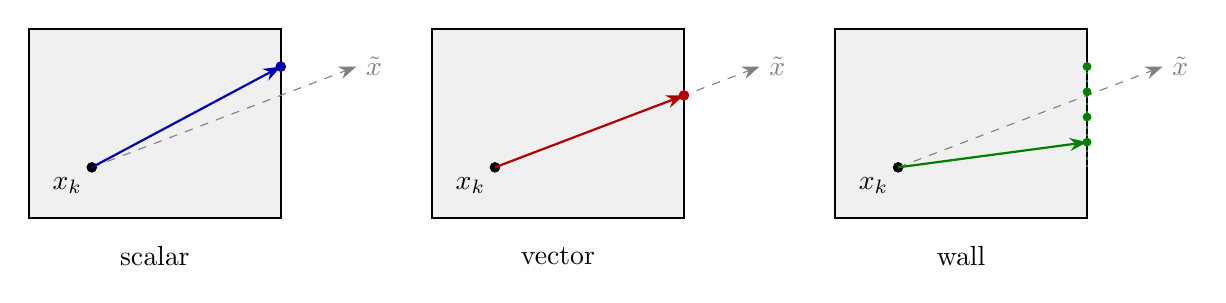
\begin{tikzpicture}[scale=1.6, >={Stealth[length=2.2mm]}]
  \foreach \xs/\name/\lab in {0/a/scalar, 3.2/b/vector, 6.4/c/wall} {
    \begin{scope}[xshift=\xs cm]
      \fill[black!6] (0,0) rectangle (2,1.5);
      \draw[thick] (0,0) rectangle (2,1.5);
      \fill (0.5,0.4) circle (1.2pt) node[below left] {$x_k$};
      \draw[->, gray, dashed] (0.5,0.4) -- (2.6,1.2) node[right] {$\tilde x$};
      \node at (1,-0.3) {\lab};
    \end{scope}
  }
  % scalar: clip x component to 2 -> (2,1.2)
  \draw[->, blue!70!black, thick] (0.5,0.4) -- (2,1.2);
  \fill[blue!70!black] (2,1.2) circle (1.2pt);
  % vector: t = (2-0.5)/2.1 = 0.714 -> (2, 0.971)
  \draw[->, red!70!black, thick] (3.7,0.4) -- (5.2,0.971);
  \fill[red!70!black] (5.2,0.971) circle (1.2pt);
  % wall: x1 on the bound for all alpha; x2 moves with alpha
  \draw[green!50!black, thick, dotted] (8.4,0.4) -- (8.4,1.2);
  \foreach \a in {0.25,0.5,0.75,1} {\fill[green!50!black] (8.4,{0.4+0.8*\a}) circle (1.0pt);}
  \draw[->, green!50!black, thick] (6.9,0.4) -- (8.4,0.6);
\end{tikzpicture}
\caption{Bounds modes for a full Newton point $\tilde x$ outside the box. Scalar: $\tilde x$ is clipped
to the box (the direction changes). Vector: the step is shortened along the Newton direction. Wall: the
clipped component is put on the bound for every trial $\alpha$ of the line search (dots), while the other
components move with $\alpha$.}
\label{fig:bounds}
\end{figure}

%=============================================================================================
\section{Convergence measures and stopping}
\label{sec:stopping}
%=============================================================================================

The size of the residual is measured by $f = \norm{F(x)}$, with the norm selected by
\code{norm\_mode}: the 2-norm (default), the $\infty$-norm $\max_i |f_i|$, or the 1-norm
$\sum_i |f_i|$. The $\infty$-norm is natural when every equation must be satisfied to a given
tolerance. The norm affects the convergence test, the reported value, the fixed-point line search,
and the uphill counter; the backtracking line search always uses the 2-norm merit function
\cref{eq:merit}, since its slope $\phi'(0)$ is defined for it.

The iteration stops with the status codes of \cref{tab:status}. Note that \code{tolx} is an absolute
tolerance on the largest change of any variable, so it should be scaled to the problem.

\begin{table}[htbp]
\centering
\caption{Status codes returned by \code{status()} (selection).}
\label{tab:status}
\small
\begin{tabular}{@{}rl@{}}
\toprule
code & meaning \\
\midrule
1 & $f \le \code{tol}$: required accuracy achieved \\
2 & $\max_i |\Delta x_i| \le \code{tolx}$: solution cannot be improved \\
3 & maximum number of iterations reached \\
4 & stopped by the user (\code{user\_input\_check}) \\
5 & more than \code{n\_uphill\_max} consecutive uphill steps \\
$-1$ to $-18$ & input errors (invalid options, missing routines, out of memory, \ldots) \\
$-1004$, $-1005$ & LSQR/LSMR/CRAIG: ill-conditioned system, iteration limit \\
$-1007$ & CRAIG: breakdown, incompatible system (use \code{damp}${}>0$) \\
$-1008$ & Cholesky: $JJ^T$ not positive definite, rank-deficient $J$ (use \code{damp}${}>0$) \\
$-1009$ & Cholesky: out of memory (envelope too large) \\
\bottomrule
\end{tabular}
\end{table}

%=============================================================================================
\section{Sparsity patterns}
\label{sec:sparsity}
%=============================================================================================

The efficiency of the sparse solvers depends on the sparsity pattern of the Jacobian, and for the
Cholesky solver on the pattern of $JJ^T$. \Cref{fig:spy} shows the patterns used in the experiments.
In the \emph{banded} problem each equation $i$ involves $9$ consecutive variables centered at column
$\approx i\, n/m$; the equations can be numbered in any order (\emph{shuffled}), which scatters the
nonzeros of $JJ^T$, but RCM recovers the band. In the \emph{grid} problem each equation is a 5-point
stencil on a $k \times k$ grid (plus one extra ``control'' variable per equation), as in a discretized
2-D PDE; then $JJ^T$ is a 13-point stencil, and after RCM its envelope (shaded) has a width of about
$2k = 2\sqrt{m}$ and contains many zeros.

% sparsity pattern plot: {file}{ncols}{nrows}{title}{mark size}
\newcommand{\spyplot}[5]{%
\begin{tikzpicture}
\begin{axis}[spy, xmax=#2+0.5, ymax=#3+0.5, title={#4}]
  \addplot[blue!70!black, only marks, mark=square*, mark size=#5] table[x=col,y=row,col sep=comma] {#1};
\end{axis}
\end{tikzpicture}}
% pattern of a square matrix with its envelope shaded: {file}{n}{envelope polygon file}{title}{mark size}
\newcommand{\spyenv}[5]{%
\begin{tikzpicture}
\begin{axis}[spy, xmax=#2+0.5, ymax=#2+0.5, title={#4}]
  \addplot[fill=orange!30, draw=orange!70!black, thin] table[x=x,y=y,col sep=comma] {#3} -- cycle;
  \addplot[blue!70!black, only marks, mark=square*, mark size=#5] table[x=col,y=row,col sep=comma] {#1};
\end{axis}
\end{tikzpicture}}

\begin{figure}[htbp]
\centering
\begin{subfigure}{0.48\textwidth}\centering
  \spyplot{data/spy_band_A.csv}{60}{36}{banded $J$ ($36\times 60$)}{1.1pt}
\end{subfigure}\hfill
\begin{subfigure}{0.48\textwidth}\centering
  \spyplot{data/spy_shuffled_A.csv}{60}{36}{shuffled $J$}{1.1pt}
\end{subfigure}\\[0.8em]
\begin{subfigure}{0.40\textwidth}\centering
  \spyplot{data/spy_shuffled_AAt.csv}{36}{36}{$JJ^T$ (shuffled order)}{1.5pt}
\end{subfigure}\hfill
\begin{subfigure}{0.40\textwidth}\centering
  \spyenv{data/spy_shuffled_AAt_rcm.csv}{36}{data/spy_shuffled_env_poly.csv}{$JJ^T$ after RCM, with envelope}{1.5pt}
\end{subfigure}\\[0.8em]
\begin{subfigure}{0.48\textwidth}\centering
  \spyplot{data/spy_grid_A.csv}{72}{36}{grid $J$ ($k=6$: $36\times 72$)}{0.9pt}
\end{subfigure}\hfill
\begin{subfigure}{0.40\textwidth}\centering
  \spyenv{data/spy_grid_AAt_rcm.csv}{36}{data/spy_grid_env_poly.csv}{grid $JJ^T$ after RCM, with envelope}{1.5pt}
\end{subfigure}
\caption{Sparsity patterns of the test problems (small instances). Top: the banded Jacobian,
and the same equations numbered in random order. Middle: the pattern of $JJ^T$ for the shuffled
Jacobian, before and after the RCM reordering of the Cholesky solver. Bottom: the 2-D grid Jacobian
and its $JJ^T$ after RCM. The shaded region is the envelope of the Cholesky factor: every entry inside it
is stored and computed, including the zeros.}
\label{fig:spy}
\end{figure}

%=============================================================================================
\section{Numerical experiments}
\label{sec:experiments}
%=============================================================================================

\paragraph{Setup.} All timings are wall-clock times on a single core of an Apple M5 (Darwin arm64), compiled with GNU Fortran (conda-forge gcc 16.2.0-7) 16.2.0 using the fpm \code{release} profile, in double precision. Each time is the best of three runs for $n \le 50{,}000$ and of one run otherwise. The benchmark program is \code{docs/benchmarks/nlesolver\_benchmarks.f90}; see \code{docs/README.md} to reproduce the results.


\subsection{Test problems}
\label{sec:exp-problems}
\begin{description}
\item[Banded.] $m$ equations, $n$ variables. Equation $i$ involves the $9$ variables
$x_{c_i-4}, \ldots, x_{c_i+4}$ with $c_i \approx 1 + (i-1)(n-1)/(m-1)$:
\begin{equation}
  f_i(x) = \sum_{j=-4}^{4} a_{ij}\, x_{c_i+j} + 0.1\, x_{c_i}^3 + 0.2 \sin(x_{c_i-4}) - b_i ,
\end{equation}
with $a_{i0} = d_0 + \sin i$ and $a_{ij} = -(1 + 0.25\cos(i+j))/|j|$ otherwise ($d_0 = 4$ unless
stated). The right-hand side is computed from a known point, so a solution exists. Underdetermined
instances use $m = 0.6\,n$; square instances $m = n$. The \emph{shuffled} variant numbers the equations in
random order.
\item[Grid.] $m = k^2$ equations, $n = 2m$ variables (a state $u$ and a control $v$ per grid node):
$f_e = 4u_e - \sum_{\text{neighbors}} u + 0.1\, u_e^3 + v_e - b_e$.
\item[Pairs.] An ill-conditioned linear test: rows $2p-1$ and $2p$ are identical except for a
perturbation $\delta$ in a separate column, so $\cond(A) \sim 1/\delta$ ($m = 400$, $n = 1000$).
\end{description}
All nonlinear runs start from $x_0 = 0$ with \code{tol}${}=10^{-10}$, and LSQR, LSMR, and CRAIG use
\code{atol}${}=$\code{btol}${}=10^{-12}$. Unless stated otherwise, the backtracking line search is
used.

\subsection{Linear solvers: underdetermined systems}
\label{sec:exp-scaling}

\Cref{fig:scaling} shows the time to solve the banded underdetermined problem for $n$ from
$10^3$ to $5\times 10^5$, and \cref{tab:scaling} gives details for $n = 50{,}000$.
All solvers that support underdetermined systems converge in three Newton iterations to the same
solution: the distance $\norm{x - x_0}$ agrees to all printed digits, confirming that they all
compute the minimum-norm step. LUSOL fails on this problem (it reports the $m \times n$ Jacobian as
singular, \cref{tab:solvers}), so it is not shown. The dense solver's cost grows like $n^3$ (3.2~s
at $n = 5{,}000$), while all the sparse solvers scale linearly with $n$. The direct Cholesky solver is
the fastest, by a factor of about 5 over CRAIG (0.14~s versus 0.65~s at $n = 500{,}000$; 2,000 times
faster than the dense solver at $n = 5{,}000$). CRAIG is 20--30\% faster than LSQR and LSMR, which use the
same bidiagonalization but do more work per iteration.

\begin{figure}[htbp]
\centering
\begin{tikzpicture}
\begin{loglogaxis}[width=0.8\textwidth, height=0.55\textwidth, xlabel={number of variables $n$ ($m = 0.6\,n$)},
  ylabel={time to solve [s]}, legend pos=south east, legend style={font=\small},
  cycle list name=solvers, grid=major, grid style={black!10}, unbounded coords=jump]
  \addplot table[x=n,y=dense,col sep=comma] {data/scaling_time.csv}; \addlegendentry{dense}
  \pgfplotsset{cycle list shift=1} % (LUSOL is not plotted: it fails for m < n)
  \addplot table[x=n,y=lsqr,col sep=comma] {data/scaling_time.csv}; \addlegendentry{LSQR}
  \addplot table[x=n,y=lsmr,col sep=comma] {data/scaling_time.csv}; \addlegendentry{LSMR}
  \addplot table[x=n,y=craig,col sep=comma] {data/scaling_time.csv}; \addlegendentry{CRAIG}
  \addplot table[x=n,y=cholesky,col sep=comma] {data/scaling_time.csv}; \addlegendentry{Cholesky}
\end{loglogaxis}
\end{tikzpicture}
\caption{Banded underdetermined problem: total time of the nonlinear solve (all Newton iterations,
function and Jacobian evaluations) versus problem size.}
\label{fig:scaling}
\end{figure}

\begin{table}[htbp]
\centering
\caption{Banded underdetermined problem, $n = 50{,}000$, $m = 30{,}000$ (backtracking line search). $\norm{x - x_0}$ is the distance from the starting point to the computed solution.}
\label{tab:scaling}
\small
\begin{tabular}{@{}llrrrrrr@{}}
\toprule
solver & status & iterations & $F$ evals & $J$ evals & $\norm{F}$ & $\norm{x-x_0}$ & time [s] \\
\midrule
LSQR & converged & 3 & 4 & 3 & $3.1\times10^{-14}$ & 28.6439 & 0.082 \\
LSMR & converged & 3 & 4 & 3 & $3.1\times10^{-14}$ & 28.6439 & 0.087 \\
CRAIG & converged & 3 & 4 & 3 & $3.1\times10^{-14}$ & 28.6439 & 0.070 \\
Cholesky & converged & 3 & 4 & 3 & $3.1\times10^{-14}$ & 28.6439 & 0.014 \\
\bottomrule
\end{tabular}
\end{table}


\subsection{Linear solvers: square systems}
\label{sec:exp-square}
For a square system the minimum-norm step is simply the Newton step, so all solvers can be compared.
\Cref{fig:square} shows the times for the square banded problem (with $d_0 = 8$, so the Jacobian is
diagonally dominant). All six solvers converge in four iterations. The two sparse direct solvers are
the fastest: Cholesky (0.35~s at $n = 500{,}000$) and LUSOL (0.43~s), followed by the iterative solvers
(1.3--1.9~s). Although the Cholesky solver is slightly faster here, it squares the condition number
(\cref{sec:exp-cond}); LUSOL factors $J$ itself and is the more robust choice for square systems that are
not well conditioned.

\begin{figure}[htbp]
\centering
\begin{tikzpicture}
\begin{loglogaxis}[width=0.8\textwidth, height=0.5\textwidth, xlabel={number of variables $n = m$},
  ylabel={time to solve [s]}, legend pos=north west, legend style={font=\small},
  cycle list name=solvers, grid=major, grid style={black!10}, unbounded coords=jump]
  \addplot table[x=n,y=dense,col sep=comma] {data/square_time.csv}; \addlegendentry{dense}
  \addplot table[x=n,y=lusol,col sep=comma] {data/square_time.csv}; \addlegendentry{LUSOL}
  \addplot table[x=n,y=lsqr,col sep=comma] {data/square_time.csv}; \addlegendentry{LSQR}
  \addplot table[x=n,y=lsmr,col sep=comma] {data/square_time.csv}; \addlegendentry{LSMR}
  \addplot table[x=n,y=craig,col sep=comma] {data/square_time.csv}; \addlegendentry{CRAIG}
  \addplot table[x=n,y=cholesky,col sep=comma] {data/square_time.csv}; \addlegendentry{Cholesky}
\end{loglogaxis}
\end{tikzpicture}
\caption{Banded square problem ($m = n$): total solve time versus problem size.}
\label{fig:square}
\end{figure}

\subsection{Step length strategies and Broyden updates}
\label{sec:exp-steps}
\Cref{tab:steps} and \cref{fig:history} compare the step-length strategies on the banded problem
($n = 50{,}000$). With the exact Jacobian, the constant step and backtracking give identical results:
from $x_0 = 0$ the full Newton step is always accepted, so backtracking costs nothing extra (the slope
$\phi'(0)$ is computed in $O(\nnz)$ operations). The exact line search needs 57 function evaluations
instead of 4 (Brent's method spends about 18 per iteration), and the fixed-point search $3 \times 5 + 1 = 16$.
On this problem the extra evaluations are cheap, but they would dominate for an expensive $F$.

With Schubert updates, the number of Jacobian evaluations drops from 3 to 1, but the number of
iterations rises from 3 to 5 (superlinear instead of quadratic convergence, \cref{fig:history}), and
the total time increases by about 70\%, because here the Jacobian is analytic and cheap and each extra
iteration costs a full linear solve. In general, saving $\Delta N_J$ Jacobian evaluations at the cost of
$\Delta N$ extra iterations pays off when
\begin{equation}
  \Delta N_J\, t_J > \Delta N\, (t_{\text{solve}} + t_F) ,
\end{equation}
where $t_J$, $t_F$, and $t_{\text{solve}}$ are the times for a Jacobian evaluation, a function evaluation, and a
linear solve. This is the case, for example, when the Jacobian is computed by finite differences.

\begin{figure}[htbp]
\centering
\begin{tikzpicture}
\begin{semilogyaxis}[width=0.48\textwidth, height=0.42\textwidth, xlabel={iteration}, xtick distance=1,
  ylabel={$\norm{F(x_k)}_2$}, title={exact Jacobian}, legend style={font=\scriptsize},
  legend pos=south west, ymin=1e-15, grid=major, grid style={black!10}]
  \addplot[blue!70!black, mark=*, mark size=1.3pt] table[x=iter,y=fnorm,col sep=comma] {data/hist_sm1_b0.csv}; \addlegendentry{constant}
  \addplot[red!70!black, mark=square, mark size=1.3pt] table[x=iter,y=fnorm,col sep=comma] {data/hist_sm2_b0.csv}; \addlegendentry{backtracking}
  \addplot[green!50!black, mark=triangle, mark size=1.5pt] table[x=iter,y=fnorm,col sep=comma] {data/hist_sm3_b0.csv}; \addlegendentry{exact}
  \addplot[orange!80!black, mark=diamond, mark size=1.5pt, dashed] table[x=iter,y=fnorm,col sep=comma] {data/hist_sm4_b0.csv}; \addlegendentry{fixed points}
\end{semilogyaxis}
\end{tikzpicture}\hfill
\begin{tikzpicture}
\begin{semilogyaxis}[width=0.48\textwidth, height=0.42\textwidth, xlabel={iteration}, xtick distance=1,
  title={Schubert (Broyden) updates}, legend style={font=\scriptsize},
  legend pos=south west, ymin=1e-15, ymax=1e5, grid=major, grid style={black!10}]
  \addplot[blue!70!black, mark=*, mark size=1.3pt] table[x=iter,y=fnorm,col sep=comma] {data/hist_sm1_b1.csv}; \addlegendentry{constant}
  \addplot[red!70!black, mark=square, mark size=1.3pt] table[x=iter,y=fnorm,col sep=comma] {data/hist_sm2_b1.csv}; \addlegendentry{backtracking}
  \addplot[green!50!black, mark=triangle, mark size=1.5pt] table[x=iter,y=fnorm,col sep=comma] {data/hist_sm3_b1.csv}; \addlegendentry{exact}
  \addplot[orange!80!black, mark=diamond, mark size=1.5pt, dashed] table[x=iter,y=fnorm,col sep=comma] {data/hist_sm4_b1.csv}; \addlegendentry{fixed points}
\end{semilogyaxis}
\end{tikzpicture}
\caption{Convergence histories for the banded problem ($n = 50{,}000$, Cholesky solver) with the
four step-length strategies, with the exact Jacobian (left) and with sparse quasi-Newton updates (right).}
\label{fig:history}
\end{figure}

\begin{table}[htbp]
\centering
\caption{Step-length strategies with and without Schubert updates, banded problem with $n = 50{,}000$.}
\label{tab:steps}
\small
\begin{tabular}{@{}lllrrrrr@{}}
\toprule
solver & step mode & updates & status & iterations & $F$ evals & $J$ evals & time [s] \\
\midrule
Cholesky & constant & no & converged & 3 & 4 & 3 & 0.013 \\
Cholesky & backtracking & no & converged & 3 & 4 & 3 & 0.014 \\
Cholesky & exact & no & converged & 3 & 57 & 3 & 0.023 \\
Cholesky & fixed points & no & converged & 3 & 16 & 3 & 0.016 \\
Cholesky & constant & yes & converged & 5 & 6 & 1 & 0.024 \\
Cholesky & backtracking & yes & converged & 5 & 6 & 1 & 0.025 \\
Cholesky & exact & yes & converged & 5 & 69 & 1 & 0.035 \\
Cholesky & fixed points & yes & converged & 5 & 26 & 1 & 0.028 \\
\midrule
CRAIG & constant & no & converged & 3 & 4 & 3 & 0.071 \\
CRAIG & backtracking & no & converged & 3 & 4 & 3 & 0.072 \\
CRAIG & exact & no & converged & 3 & 57 & 3 & 0.086 \\
CRAIG & fixed points & no & converged & 3 & 16 & 3 & 0.080 \\
CRAIG & constant & yes & converged & 5 & 6 & 1 & 0.120 \\
CRAIG & backtracking & yes & converged & 5 & 6 & 1 & 0.119 \\
CRAIG & exact & yes & converged & 5 & 69 & 1 & 0.132 \\
CRAIG & fixed points & yes & converged & 5 & 26 & 1 & 0.122 \\
\bottomrule
\end{tabular}
\end{table}


\subsection{Conditioning}
\label{sec:exp-cond}
\Cref{fig:cond} (left) shows the number of CRAIG iterations for one linear solve of the banded matrix
($n = 50{,}000$, linear part only) as the diagonal weight $d_0$ is reduced. The iteration count grows roughly
in proportion to $\cond(A)$ (from 15 to 95 iterations as $\cond(A)$ grows from 1.6 to 14), as expected from
\cref{sec:craig}, while the Cholesky solver takes the same time (about 6~ms) in every case.
Note also that the residual attained by CRAIG ($\approx 5\times10^{-8}$, i.e.\ $4\times10^{-10}$ relative to
$\norm{b}$) is larger than requested: the residual estimate $|\beta_{k+1}\zeta_k|$ drifts from the true
residual in floating point. Inside the Newton iteration this is harmless (the next iteration corrects it;
the nonlinear runs all reach $\norm{F} \approx 10^{-14}$), but it limits the accuracy of a single solve.

\Cref{fig:cond} (right) shows the accuracy of the minimum-norm solution for the ``pairs'' matrix, whose
condition number is controlled by $\delta$, relative to the LAPACK \code{dgels} solution. Without
refinement, the error of the Cholesky solver grows like $\epsilon\, \cond(A)^2$, as predicted in
\cref{sec:cholesky}. With refinement it follows $\epsilon\,\cond(A)$ (the accuracy of a backward stable
method) up to $\cond(A) \approx 4\times10^{6}$. At $\cond(A) \approx 4\times 10^7$ the refinement converges
slowly (error $7\times10^{-6}$), and beyond $\cond(A) \approx 10^{8}$ the factorization breaks down and the solver
reports a rank-deficient Jacobian (plotted as a relative error of 1). CRAIG works directly with $A$ and remains
accurate (error $\approx \epsilon\,\cond(A)$) over the whole range.

\begin{figure}[htbp]
\centering
\begin{tikzpicture}
\begin{loglogaxis}[width=0.48\textwidth, height=0.42\textwidth, xlabel={$\cond(A)$},
  ylabel={CRAIG iterations}, title={banded, $n = 50{,}000$}, grid=major, grid style={black!10},
  log ticks with fixed point, xtick={1,2,5,10,20}, ytick={10,20,50,100}]
  \addplot[red!70!black, only marks, mark=pentagon*] table[x=cond,y=craig_iters,col sep=comma] {data/cond_craig.csv};
  \addplot[gray, dashed, domain=1.5:15, samples=2] {7*x};
\end{loglogaxis}
\end{tikzpicture}\hfill
\begin{tikzpicture}
\begin{loglogaxis}[width=0.48\textwidth, height=0.42\textwidth, xlabel={$\cond(A)$},
  ylabel={relative error in $x$}, title={pairs, vs.\ LAPACK \code{dgels}},
  legend style={font=\scriptsize, at={(0.5,-0.3)}, anchor=north, legend columns=2},
  grid=major, grid style={black!10}, ymax=10]
  \addplot[red!70!black, mark=pentagon*] table[x=cond,y=err_craig,col sep=comma] {data/cond_accuracy.csv}; \addlegendentry{CRAIG}
  \addplot[green!50!black, mark=star, dashed] table[x=cond,y=err_chol0,col sep=comma] {data/cond_accuracy.csv}; \addlegendentry{Cholesky, no refinement}
  \addplot[green!50!black, mark=star, thick] table[x=cond,y=err_chol2,col sep=comma] {data/cond_accuracy.csv}; \addlegendentry{Cholesky, refinement}
  \addplot[gray, domain=1:1e10, samples=2] {2.2e-16*x}; \addlegendentry{$\epsilon\,\cond(A)$}
  \addplot[gray, dashed, domain=1:1e8, samples=2] {2.2e-16*x^2}; \addlegendentry{$\epsilon\,\cond(A)^2$}
\end{loglogaxis}
\end{tikzpicture}
\caption{Left: CRAIG iterations for one linear solve versus the condition number of the banded matrix
(varying the diagonal weight $d_0$; dashed: $7\,\cond(A)$). Right: accuracy of the minimum-norm solution for the ill-conditioned
``pairs'' matrix.}
\label{fig:cond}
\end{figure}

\subsection{Effect of the sparsity pattern}
\label{sec:exp-sparsity}
\Cref{tab:sparsity} and \cref{fig:grid} show how the sparsity pattern affects the Cholesky solver.
Numbering the equations of the banded problem in random order raises the bandwidth of $JJ^T$ from 7 to
29,922, but RCM recovers a bandwidth of 7 and the same envelope; the solve is only about 35\% slower,
because the rows of $J$ are now scattered in memory.

For the 2-D grid problem, the bandwidth of $JJ^T$ is $2k = 2\sqrt{m}$ in the natural order, and RCM cannot reduce
it. The envelope grows like $1.35\, m^{1.5}$ and the work like $m^2$: the Cholesky time grows from
0.8~ms at $m = 625$ to 2.4~s at $m = 40{,}000$, while CRAIG grows almost linearly. CRAIG becomes faster than the
Cholesky solver between $m = 2{,}500$ and $m = 10{,}000$, and is 7.6 times faster at $m = 40{,}000$. A general
sparse Cholesky factorization with a fill-reducing ordering would remove most of this growth (\cref{sec:future}).

\begin{figure}[htbp]
\centering
\begin{tikzpicture}
\begin{loglogaxis}[width=0.48\textwidth, height=0.42\textwidth, xlabel={number of equations $m = k^2$},
  ylabel={envelope size of $L$}, title={grid problem}, legend style={font=\scriptsize},
  legend pos=north west, grid=major, grid style={black!10}]
  \addplot[green!50!black, mark=star, thick] table[x=m,y=envelope,col sep=comma,
     restrict expr to domain={\thisrow{param}}{1:1000}] {data/sparsity.csv}; \addlegendentry{envelope}
  \addplot[gray, dashed, domain=600:40000, samples=2] {1.35*x^1.5}; \addlegendentry{$1.35\,m^{1.5}$}
\end{loglogaxis}
\end{tikzpicture}\hfill
\begin{tikzpicture}
\begin{loglogaxis}[width=0.48\textwidth, height=0.42\textwidth, xlabel={number of equations $m = k^2$},
  ylabel={time to solve [s]}, title={grid problem}, legend style={font=\scriptsize},
  legend pos=north west, grid=major, grid style={black!10}]
  \addplot[green!50!black, mark=star, thick] table[x=m,y=chol_time,col sep=comma,
     restrict expr to domain={\thisrow{param}}{1:1000}] {data/sparsity.csv}; \addlegendentry{Cholesky}
  \addplot[red!70!black, mark=pentagon*] table[x=m,y=craig_time,col sep=comma,
     restrict expr to domain={\thisrow{param}}{1:1000}] {data/sparsity.csv}; \addlegendentry{CRAIG}
\end{loglogaxis}
\end{tikzpicture}
\caption{Grid problem: the envelope of the Cholesky factor grows like $m^{1.5}$ (left), so the
Cholesky solver loses its advantage over CRAIG as the grid is refined (right).}
\label{fig:grid}
\end{figure}

\begin{table}[htbp]
\centering
\caption{Effect of the sparsity pattern on the Cholesky solver: bandwidth of $JJ^T$ in the given order and after RCM, envelope size of $L$, and total solve times (Cholesky and CRAIG).}
\label{tab:sparsity}
\small
\begin{tabular}{@{}lrrrrrrr@{}}
\toprule
problem & $n$ & $m$ & bandwidth & after RCM & envelope & Cholesky [s] & CRAIG [s] \\
\midrule
banded & 50{,}000 & 30{,}000 & 7 & 7 & 169{,}992 & 0.014 & 0.071 \\
shuffled & 50{,}000 & 30{,}000 & 29{,}922 & 7 & 169{,}992 & 0.019 & 0.074 \\
grid{,} $k=25$ & 1{,}250 & 625 & 50 & 50 & 21{,}963 & 0.0008 & 0.0050 \\
grid{,} $k=50$ & 5{,}000 & 2{,}500 & 100 & 100 & 171{,}425 & 0.0086 & 0.021 \\
grid{,} $k=100$ & 20{,}000 & 10{,}000 & 200 & 200 & 1{,}352{,}850 & 0.127 & 0.086 \\
grid{,} $k=150$ & 45{,}000 & 22{,}500 & 300 & 300 & 4{,}544{,}275 & 0.698 & 0.172 \\
grid{,} $k=200$ & 80{,}000 & 40{,}000 & 400 & 400 & 10{,}745{,}700 & 2.36 & 0.310 \\
\bottomrule
\end{tabular}
\end{table}


%=============================================================================================
\section{Recommended settings}
\label{sec:recommendations}
%=============================================================================================

\Cref{tab:recommend} suggests a linear solver for common types of problems, based on the analysis of
\cref{sec:linear} and the experiments of \cref{sec:experiments}. The other options are discussed below.

\begin{table}[htbp]
\centering
\caption{Suggested linear solver (\code{sparsity\_mode}) by problem type.}
\label{tab:recommend}
\small
\begin{tabular}{@{}p{0.42\textwidth}p{0.53\textwidth}@{}}
\toprule
problem & suggested solver \\
\midrule
small ($n \lesssim 2{,}000$), any shape & dense (1) \\
square, sparse & LUSOL (3); Cholesky (7) if well conditioned and (mostly) banded \\
underdetermined, sparse, banded or mostly banded (in any numbering) & Cholesky (7) \\
underdetermined, sparse, 2-D/3-D mesh-like or irregular coupling & CRAIG (6), or an external sparse QR (e.g.\ qr\_mumps) via mode 5 \\
underdetermined, ill-conditioned ($\cond(J) \gtrsim 10^7$) & CRAIG (6), or Cholesky (7) with \code{damp}${}>0$ \\
rank-deficient or nearly singular Jacobian & CRAIG (6), Cholesky (7), LSQR (2), or LSMR (4) with \code{damp}${}>0$ \\
overdetermined (least squares), sparse & LSQR (2) or LSMR (4) \\
\bottomrule
\end{tabular}
\end{table}

\paragraph{Step length.} Use backtracking (\code{step\_mode=2}) as the default: it accepts the full Newton
step whenever that step decreases $\norm{F}$ sufficiently, so it costs nothing when the full step works, and
it protects against divergence from a poor starting point. Keep \code{backtrack\_c} small (the default
$10^{-4}$; it must be below $0.5$). The constant step (mode 1) with $\code{alpha} = 1$ is pure Newton and is
appropriate when the starting point is known to be good. The fixed-point (mode 4) and exact (mode 3) searches
are more thorough per iteration, which can help on difficult problems when $F$ is cheap, but they cost about 5
and 15--20 function evaluations per iteration.

\paragraph{Broyden updates.} Use \code{use\_broyden=.true.} only when a Jacobian evaluation is expensive
compared with a function evaluation plus a linear solve, for example a finite-difference Jacobian or a costly
simulation. Combine it with backtracking: full quasi-Newton steps without a line search can diverge. Values of
\code{broyden\_update\_n} between 3 and 10 are reasonable; smaller values re-evaluate the Jacobian more often.

\paragraph{Iterative solver tolerances.} For LSQR, LSMR, and CRAIG, set \code{atol} and \code{btol} to
$10^{-10}$--$10^{-12}$ and \code{itnlim} to a few times the expected number of iterations (it is 100 by default,
which is too small for large ill-conditioned problems). Since the Newton iteration corrects an inexact step,
looser tolerances (e.g.\ $10^{-6}$) can also be used far from the solution, at the cost of more Newton iterations.

\paragraph{Damping.} Use \code{damp}${}>0$ (a small multiple of the expected size of the Jacobian entries,
e.g.\ $10^{-6}$ to $10^{-3}$ times it) when the Jacobian may lose rank. Larger values give shorter, more
conservative steps, and reduce the convergence rate near the solution.

\paragraph{Bounds.} The vector mode keeps the Newton direction and is the natural choice when the bounds are
rarely active. When some variables are often at their bounds, the scalar or wall modes let the other variables
keep moving; the wall mode also keeps the bounded variables fixed during the line search.

\paragraph{Norms and tolerances.} Use the $\infty$-norm when every equation must be satisfied to a given absolute
tolerance, and the 2-norm otherwise. Scale the variables and equations so that their typical values are of order
one: this makes \code{tol}, \code{tolx}, and the damping parameter meaningful, and improves the conditioning of
the Jacobian, which matters for all the iterative solvers and for the Cholesky solver.

\paragraph{Example.} A good starting point for a large, sparse, underdetermined problem:
\begin{lstlisting}
call solver%initialize(n=n, m=m, max_iter=50, tol=1.0e-10_wp, tolx=1.0e-12_wp, &
                       func=func, grad_sparse=grad_sparse, irow=irow, icol=icol, &
                       sparsity_mode = NLESOLVER_SPARSITY_CHOLESKY, &   ! or _CRAIG
                       step_mode     = NLESOLVER_LINESEARCH_BACKTRACKING, &
                       norm_mode     = NLESOLVER_2_NORM)
\end{lstlisting}

%=============================================================================================
\section{Limitations and possible extensions}
\label{sec:future}
%=============================================================================================

\begin{itemize}
  \item \textbf{General sparsity in the direct solver.} The envelope storage of mode 7 is ideal for
  banded Jacobians, but for mesh-like sparsity a fill-reducing ordering (approximate minimum degree
  \cite{amd} or nested dissection) with a general (supernodal) sparse Cholesky factorization would
  reduce the factorization work from about $O(m^2)$ to $O(m^{1.5})$ for 2-D problems.
  \item \textbf{Closest solution.} An ``anchored'' step (\cref{sec:newton}) would converge to the
  solution closest to $x_0$ (or to a reference point, optionally weighted), which is often what is
  wanted for underdetermined problems (e.g.\ the smallest correction to a nominal design). It converges
  only linearly, since it ignores the curvature of $\mathcal{M}$, and needs a modified stopping test.
  \item \textbf{Inexact Newton.} The tolerances of the iterative solvers could be tied to $\norm{F_k}$
  (Eisenstat--Walker forcing terms), avoiding needlessly accurate steps far from the solution.
  \item \textbf{Finite-difference Jacobians} with column grouping (Curtis--Powell--Reid) for sparse
  problems, and an adaptive damping parameter (Levenberg--Marquardt or trust region) for robustness far
  from the solution.
  \item \textbf{Conditioning.} Mode 7 is reliable for $\cond(J) \lesssim 10^8$; a sparse QR factorization of
  $J^T$ would remove this limit at a higher cost.
\end{itemize}

%=============================================================================================
\appendix
\section{Interface summary}
\label{sec:api}
%=============================================================================================

The solver is a class, \code{nlesolver\_type}, with the methods \code{initialize}, \code{solve},
\code{status}, and \code{destroy}. A minimal sparse example:
\begin{lstlisting}
use nlesolver_module
type(nlesolver_type) :: solver
call solver%initialize(n=n, m=m, max_iter=50, tol=1.0e-10_nlesolver_rk, &
                       func=func, grad_sparse=grad_sparse,               &
                       sparsity_mode=NLESOLVER_SPARSITY_CHOLESKY,        &
                       irow=irow, icol=icol,                             &
                       step_mode=NLESOLVER_LINESEARCH_BACKTRACKING)
call solver%solve(x)          ! x: initial guess on input, solution on output
call solver%status(istat, message)
\end{lstlisting}
\Cref{tab:options} lists the options of \code{initialize}.

\begin{table}[h]
\centering
\caption{Options of \code{initialize} (defaults in parentheses).}
\label{tab:options}
\small
\begin{tabular}{@{}p{0.27\textwidth}p{0.68\textwidth}@{}}
\toprule
option & description \\
\midrule
\code{n}, \code{m} & number of variables and equations \\
\code{func}, \code{grad}, \code{grad\_sparse} & function, dense Jacobian, sparse Jacobian (values in the order of \code{irow}/\code{icol}) \\
\code{max\_iter}, \code{tol}, \code{tolx} & iteration limit, tolerance on $\norm{F}$, tolerance on $\max|\Delta x_i|$ ($10^{-8}$) \\
\code{norm\_mode} & 1: 2-norm (default), 2: $\infty$-norm, 3: 1-norm \\
\code{step\_mode} & 1: constant (default), 2: backtracking, 3: exact, 4: fixed points \\
\code{alpha}, \code{alpha\_min}, \code{alpha\_max} & constant step (1); step limits (0.1, 1) \\
\code{backtrack\_c}, \code{backtrack\_tau} & Armijo constant ($10^{-4}$), reduction factor (0.5) \\
\code{fmin\_tol}, \code{n\_intervals} & exact line search tolerance ($10^{-5}$); fixed-point intervals (2) \\
\code{use\_broyden}, \code{broyden\_update\_n} & quasi-Newton updates (false); updates between resets (4) \\
\code{n\_uphill\_max} & maximum consecutive uphill steps (5) \\
\code{sparsity\_mode} & linear solver, \cref{tab:solvers} (1: dense) \\
\code{irow}, \code{icol} & sparsity pattern (sparse modes) \\
\code{atol}, \code{btol}, \code{conlim}, \code{itnlim} & LSQR/LSMR/CRAIG stopping parameters (0, 0, 0, 100) \\
\code{damp} & damping $\delta$ for modes 2, 4, 6, 7 (0) \\
\code{localSize} & LSMR reorthogonalization vectors (0) \\
\code{lusol\_method} & LUSOL pivoting: 0 partial, 1 rook, 2 complete (0) \\
\code{cholesky\_refine} & mode 7 refinement steps (2) \\
\code{custom\_solver\_sparse} & user linear solver (mode 5) \\
\code{bounds\_mode}, \code{xlow}, \code{xupp} & bounds handling, \cref{sec:bounds} (0: ignore) \\
\code{export\_iteration}, \code{user\_input\_check} & callbacks for output and user stop \\
\code{verbose}, \code{iunit} & diagnostic output \\
\bottomrule
\end{tabular}
\end{table}

%=============================================================================================
\begin{thebibliography}{99}
\bibitem{dennis_schnabel} J.~E. Dennis and R.~B. Schnabel, \emph{Numerical Methods for Unconstrained
Optimization and Nonlinear Equations}, SIAM, 1996.
\bibitem{benisrael1966} A.~Ben-Israel, ``A Newton--Raphson method for the solution of systems of
equations'', \emph{J. Math. Anal. Appl.} 15 (1966), 243--252.
\bibitem{levin_benisrael} Y.~Levin and A.~Ben-Israel, ``A Newton method for systems of $m$ equations in
$n$ variables'', \emph{Nonlinear Analysis} 47 (2001), 1961--1971.
\bibitem{lsqr} C.~C. Paige and M.~A. Saunders, ``LSQR: An algorithm for sparse linear equations and
sparse least squares'', \emph{ACM Trans. Math. Softw.} 8 (1982), 43--71.
\bibitem{lsmr} D.~C.-L. Fong and M.~A. Saunders, ``LSMR: An iterative algorithm for sparse
least-squares problems'', \emph{SIAM J. Sci. Comput.} 33 (2011), 2950--2971.
\bibitem{saunders1995} M.~A. Saunders, ``Solution of sparse rectangular systems using LSQR and CRAIG'',
\emph{BIT} 35 (1995), 588--604.
\bibitem{lusol} P.~E. Gill, W.~Murray, M.~A. Saunders, and M.~H. Wright, ``Maintaining LU factors of a
general sparse matrix'', \emph{Linear Algebra Appl.} 88/89 (1987), 239--270.
\bibitem{cuthill_mckee} E.~Cuthill and J.~McKee, ``Reducing the bandwidth of sparse symmetric
matrices'', \emph{Proc. 24th ACM National Conference} (1969), 157--172.
\bibitem{george_liu} A.~George and J.~W.~H. Liu, \emph{Computer Solution of Large Sparse Positive
Definite Systems}, Prentice-Hall, 1981.
\bibitem{bjorck} \AA.~Bj\"orck, \emph{Numerical Methods for Least Squares Problems}, SIAM, 1996.
\bibitem{brent} R.~P. Brent, \emph{Algorithms for Minimization without Derivatives}, Prentice-Hall, 1973.
\bibitem{broyden} C.~G. Broyden, ``A class of methods for solving nonlinear simultaneous equations'',
\emph{Math. Comp.} 19 (1965), 577--593.
\bibitem{schubert} L.~K. Schubert, ``Modification of a quasi-Newton method for nonlinear equations with
a sparse Jacobian'', \emph{Math. Comp.} 24 (1970), 27--30.
\bibitem{amd} P.~R. Amestoy, T.~A. Davis, and I.~S. Duff, ``An approximate minimum degree ordering
algorithm'', \emph{SIAM J. Matrix Anal. Appl.} 17 (1996), 886--905.
\bibitem{qrmumps} E.~Agullo, A.~Buttari, A.~Guermouche, and F.~Lopez, ``Implementing multifrontal sparse
solvers for multicore architectures with sequential task flow runtime systems'', \emph{ACM Trans. Math.
Softw.} 43 (2016), 13:1--13:22.
\end{thebibliography}

\end{document}
